\documentclass[11pt,a4paper]{article}
\usepackage[margin=0.78in,headheight=14pt,footskip=24pt]{geometry}
\usepackage[T1]{fontenc}
\usepackage{lmodern}
\usepackage{xcolor}
\usepackage{listings}
\usepackage{graphicx}
\usepackage{float}
\usepackage{fancyhdr}
\usepackage{booktabs}
\usepackage{caption}
\usepackage{titlesec}
\usepackage{microtype}
\usepackage{amsmath}
\usepackage{enumitem}
\usepackage{array}

\definecolor{codebg}{RGB}{247,247,247}
\definecolor{codegreen}{RGB}{0,110,55}
\definecolor{codeblue}{RGB}{30,70,160}
\definecolor{codepurple}{RGB}{135,40,140}
\lstdefinestyle{terminalstyle}{
  basicstyle=\ttfamily\scriptsize,
  backgroundcolor=\color{codebg},
  breaklines=true,
  frame=single,
  rulecolor=\color{black!18},
  columns=fullflexible,
  keepspaces=true,
  showstringspaces=false
}
\lstdefinestyle{pythonstyle}{
  language=Python,
  basicstyle=\ttfamily\scriptsize,
  backgroundcolor=\color{codebg},
  keywordstyle=\color{codeblue}\bfseries,
  commentstyle=\color{codegreen}\itshape,
  stringstyle=\color{codepurple},
  breaklines=true,
  frame=single,
  rulecolor=\color{black!18},
  numbers=left,
  numberstyle=\tiny\color{gray},
  numbersep=6pt,
  columns=fullflexible,
  showstringspaces=false
}
\pagestyle{fancy}
\fancyhf{}
\lhead{}
\rhead{\small Big Data Analysis Lab}
\rfoot{\small Experiment 8}
\cfoot{\thepage}
\renewcommand{\headrulewidth}{0.4pt}
\setlength{\parindent}{0pt}
\setlength{\parskip}{4pt}
\titleformat{\section}{\large\bfseries}{\thesection}{0.7em}{}
\titleformat{\subsection}{\normalsize\bfseries}{\thesubsection}{0.7em}{}
\captionsetup{font=small,labelfont=bf}
\setlength{\intextsep}{5pt}
\setlength{\textfloatsep}{5pt}
\setlength{\abovecaptionskip}{3pt}
\setlength{\belowcaptionskip}{0pt}

\begin{document}
\noindent
\textbf{Name:} Nikhil Sunchu\\
\textbf{Class:} D20A-31

\vspace{0.5em}
\begin{center}
{\Large\bfseries Experiment 8: Installation and Use of HBase}\\
\textbf{Creating a NoSQL Table, Loading Data, Querying Records, and Visualization}
\end{center}

\section*{Aim}
To install and configure a NoSQL database environment and perform table creation, data loading, query execution, and visualization using HBase.

\section{Theory}
HBase is a distributed, column-oriented NoSQL database built on top of Hadoop HDFS. It is designed to store and retrieve large datasets using row keys and column families. Unlike a relational database, HBase does not require a fixed schema for every individual column; columns are grouped into column families defined when a table is created.

\textbf{Table and row key:} An HBase table contains rows identified by unique row keys. In this experiment, each student ID (for example, \texttt{S101}) is used as the row key.

\textbf{Column families:} The \texttt{students} table uses two column families. The \texttt{info} family stores student name, department, and semester. The \texttt{marks} family stores subject and score.

\textbf{HBase Shell:} The shell provides commands such as \texttt{create}, \texttt{describe}, \texttt{put}, \texttt{scan}, \texttt{get}, and \texttt{count} to manage tables and retrieve records.

\textbf{Visualization:} The student records were exported to a CSV file and plotted using Python's Matplotlib library. A bar chart compares each student's marks in Big Data.

\section{Experimental Procedure and Results}

\subsection{1. Verify HBase Services}
The running HBase processes were checked from the Cloudera QuickStart environment using the following command.
\begin{lstlisting}[style=terminalstyle]
sudo -u hbase jps
\end{lstlisting}
The output showed the HBase Master, RegionServer, ThriftServer, and RESTServer processes. This confirmed that the required HBase services were running.
\begin{figure}[H]
\centering
\includegraphics[width=0.60\linewidth]{hbase_services.png}
\caption{HBase services running in the Cloudera environment.}
\end{figure}

\subsection{2. Create and Describe the Table}
The HBase table named \texttt{students} was created with two column families, \texttt{info} and \texttt{marks}. The table configuration was verified using:
\begin{lstlisting}[style=terminalstyle]
describe 'students'
\end{lstlisting}
The table was enabled and the description showed both column families.
\begin{figure}[H]
\centering
\includegraphics[width=0.86\linewidth]{table_description.png}
\caption{Description of the students table and its column families.}
\end{figure}

\subsection{3. Load and Display Student Data}
Ten student records were stored in the \texttt{students} table. The \texttt{info} family contains each student's name, department, and semester. The \texttt{marks} family contains the subject and score. The full table was displayed using:
\begin{lstlisting}[style=terminalstyle]
scan 'students'
\end{lstlisting}
\begin{figure}[H]
\centering
\includegraphics[width=0.94\linewidth]{full_scan.png}
\caption{All 10 student records retrieved from HBase.}
\end{figure}

\subsection{4. Execute HBase Queries}
\textbf{Retrieve a single row:} The record for student \texttt{S101} was retrieved using:
\begin{lstlisting}[style=terminalstyle]
get 'students', 'S101'
\end{lstlisting}
The returned record contained the student's department, name, semester, subject, and score.
\begin{figure}[H]
\centering
\includegraphics[width=0.78\linewidth]{get_student.png}
\caption{Retrieving the record for student S101.}
\end{figure}

\textbf{Select specific columns:} Only student names and marks were requested with:
\begin{lstlisting}[style=terminalstyle]
scan 'students', {COLUMNS => ['info:name', 'marks:score']}
\end{lstlisting}
The query returned names and scores for all 10 students.
\begin{figure}[H]
\centering
\includegraphics[width=0.94\linewidth]{selected_columns.png}
\caption{Selecting the name and score columns from the table.}
\end{figure}

\textbf{Filter by department:} The following filter returned only students whose department is IT:
\begin{lstlisting}[style=terminalstyle]
scan 'students', {FILTER => "SingleColumnValueFilter('info', 'department', =, 'binary:IT')"}
\end{lstlisting}
The query returned four records: S101 (Nikhil), S103 (Amit), S106 (Anjali), and S109 (Arjun).
\begin{figure}[H]
\centering
\includegraphics[width=0.94\linewidth]{department_filter.png}
\caption{Filtering student records by the IT department.}
\end{figure}

\subsection{5. Export Data to CSV}
The HBase shell output was converted into a structured CSV dataset named \texttt{students.csv}. It contains six fields: student ID, name, department, semester, subject, and score. A representative portion of the file is shown below.
\begin{lstlisting}[style=terminalstyle]
student_id,name,department,semester,subject,score
S101,Nikhil,IT,6,Big Data,85
S102,Priya,CSE,6,Big Data,91
S103,Amit,IT,6,Big Data,76
S104,Sneha,CSE,6,Big Data,88
S105,Rohan,AIDS,6,Big Data,79
... (10 student records in total)
\end{lstlisting}
The CSV file was used as the input dataset for visualization.

\subsection{6. Visualize Student Marks Using Matplotlib}
Python and Matplotlib were used to read the CSV file and create a bar chart. Student names are displayed on the horizontal axis and marks on the vertical axis. The vertical scale ranges from 0 to 100, and each bar is labelled with the student's score. The chart was saved as \texttt{student\_marks.png}.
\begin{lstlisting}[style=pythonstyle]
import csv
import matplotlib.pyplot as plt

names = []
scores = []
with open("students.csv", newline="") as file:
    reader = csv.DictReader(file)
    for row in reader:
        names.append(row["name"])
        scores.append(int(row["score"]))

plt.figure(figsize=(10, 6))
bars = plt.bar(names, scores)
plt.title("Big Data Marks of Students")
plt.xlabel("Student Name")
plt.ylabel("Marks")
plt.ylim(0, 100)
plt.grid(axis="y", linestyle="--", alpha=0.4)
for bar, score in zip(bars, scores):
    plt.text(bar.get_x() + bar.get_width()/2,
             bar.get_height() + 1, str(score), ha="center")
plt.tight_layout()
plt.savefig("student_marks.png", dpi=300)
plt.show()
\end{lstlisting}
\begin{figure}[H]
\centering
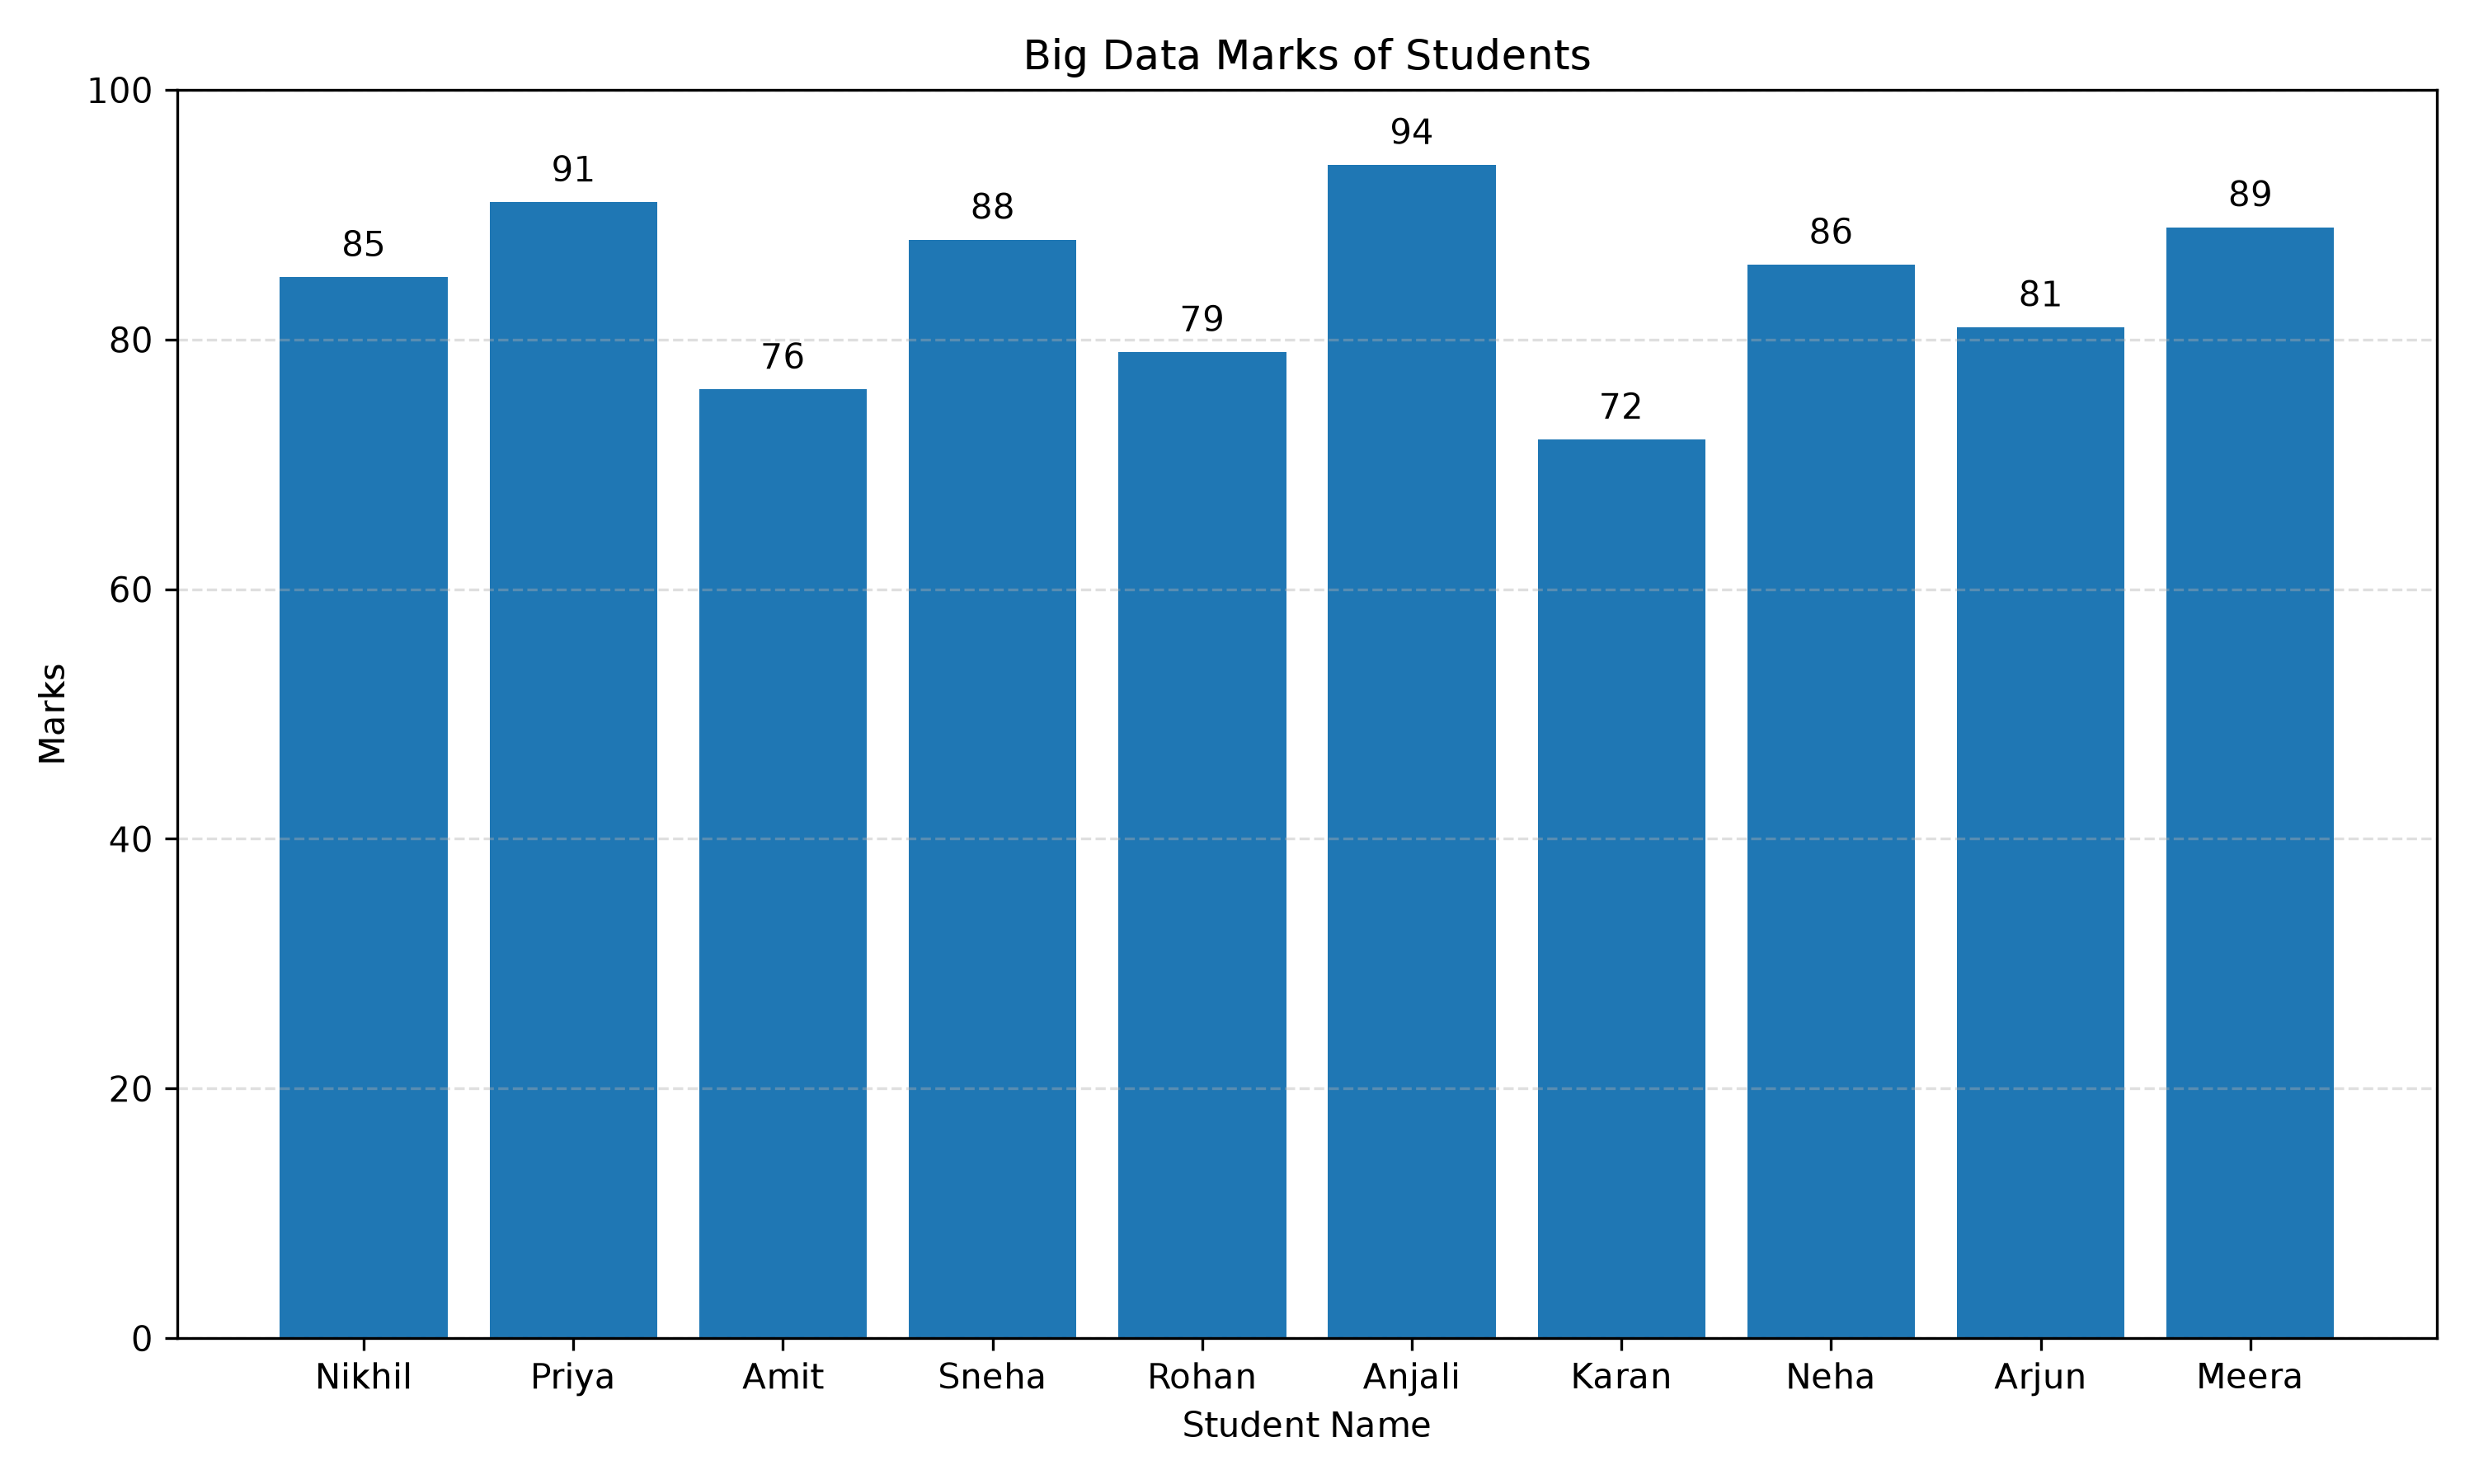
\includegraphics[width=0.94\linewidth]{student_marks.png}
\caption{Bar chart comparing the Big Data marks of 10 students.}
\end{figure}

\section{Observation}
\begin{center}
\begin{tabular}{>{\raggedright\arraybackslash}p{0.62\linewidth}p{0.27\linewidth}}
\toprule
\textbf{Operation} & \textbf{Observation} \\
\midrule
HBase services & Running \\
Table configuration & \texttt{students} enabled; two column families \\
Data loading & 10 student records \\
Single-row retrieval & Successful for S101 \\
Column selection & Names and marks returned \\
Department filter & 4 IT students returned \\
CSV preparation & 10 records with 6 fields \\
Matplotlib visualization & Chart generated and saved \\
\bottomrule
\end{tabular}
\end{center}

\section{Conclusion}
The experiment demonstrated the use of HBase as a NoSQL database for storing and retrieving student-performance data. The \texttt{students} table was configured with the \texttt{info} and \texttt{marks} column families, and 10 records were queried using row retrieval, column selection, and a department filter. The records were then organized into a CSV file and visualized using Matplotlib. The experiment covered table configuration, data loading, NoSQL query operations, and data visualization.

\end{document}
